\documentclass[12pt,a4paper,oneside]{report}

% -------------------------------------------------------------------
% Editable title-page details
% -------------------------------------------------------------------
\newcommand{\studentname}{[Student Name]}
\newcommand{\rollnumber}{[Roll Number]}
\newcommand{\supervisor}{[Project Supervisor]}
\newcommand{\projectcourse}{Undergraduate Project Report (MTH496)}
\newcommand{\department}{Department of Mathematics and Statistics}
\newcommand{\institution}{Indian Institute of Technology, Kanpur}
\newcommand{\projecttitle}{Mathematical Modelling and Forecasting of Agricultural Mandi Prices\ using an Adaptive Kalman Filter}

\usepackage[a4paper,margin=1in]{geometry}
\usepackage{amsmath,amssymb,amsfonts,amsthm,mathtools}
\usepackage{graphicx}
\usepackage{booktabs}
\usepackage{array}
\usepackage{longtable}
\usepackage{enumitem}
\usepackage{float}
\usepackage{caption}
\usepackage{subcaption}
\usepackage{hyperref}
\usepackage{microtype}
\usepackage{fancyhdr}
\usepackage{listings}
\usepackage{xcolor}
\usepackage{url}
\usepackage{setspace}
\usepackage{titlesec}
\graphicspath{{figures/}}

\hypersetup{hidelinks,bookmarksnumbered=true,pdfauthor={\studentname},pdftitle={\projecttitle}}
\setstretch{1.10}\setlength{\headheight}{14pt}
\setlength{\parskip}{0.35em}
\setlength{\parindent}{1.5em}
\setlist[itemize]{leftmargin=2em,itemsep=0.2em,topsep=0.25em}
\setlist[enumerate]{leftmargin=2em,itemsep=0.25em,topsep=0.25em}
\captionsetup{font=small,labelfont=bf}
\numberwithin{equation}{chapter}
\numberwithin{figure}{chapter}
\numberwithin{table}{chapter}

\pagestyle{fancy}
\fancyhf{}
\fancyhead[L]{\small Agricultural Mandi Price Forecasting}
\fancyhead[R]{\small Undergraduate Project Report}
\fancyfoot[C]{\thepage}
\renewcommand{\headrulewidth}{0.4pt}

\theoremstyle{definition}
\newtheorem{definition}{Definition}[chapter]
\newtheorem{example}{Example}[chapter]
\newtheorem{remark}{Remark}[chapter]
\theoremstyle{plain}
\newtheorem{proposition}{Proposition}[chapter]
\newtheorem{theorem}{Theorem}[chapter]

\DeclareMathOperator{\Var}{Var}
\DeclareMathOperator{\Cov}{Cov}
\DeclareMathOperator{\E}{E}
\DeclareMathOperator{\diag}{diag}
\DeclareMathOperator{\tr}{tr}
\DeclareMathOperator{\argmin}{arg\,min}
\newcommand{\R}{\mathbb{R}}
\newcommand{\1}{\mathbf{1}}
\newcommand{\trans}{^{\mathsf T}}
\newcommand{\given}{\,\mid\,}
\newcommand{\hatt}[1]{\widehat{#1}}
\newcommand{\Rs}{\text{Rs.}}
\newcommand{\dd}{\,\mathrm{d}}

\lstset{
  basicstyle=\ttfamily\small,
  columns=fullflexible,
  keepspaces=true,
  breaklines=true,
  frame=single,
  rulecolor=\color{black!30},
  showstringspaces=false,
  keywordstyle=\bfseries,
  commentstyle=\itshape\color{black!65}
}

\begin{document}

% =============================== TITLE ===============================
\begin{titlepage}
\thispagestyle{empty}

\centering
\IfFileExists{logo.png}{%
  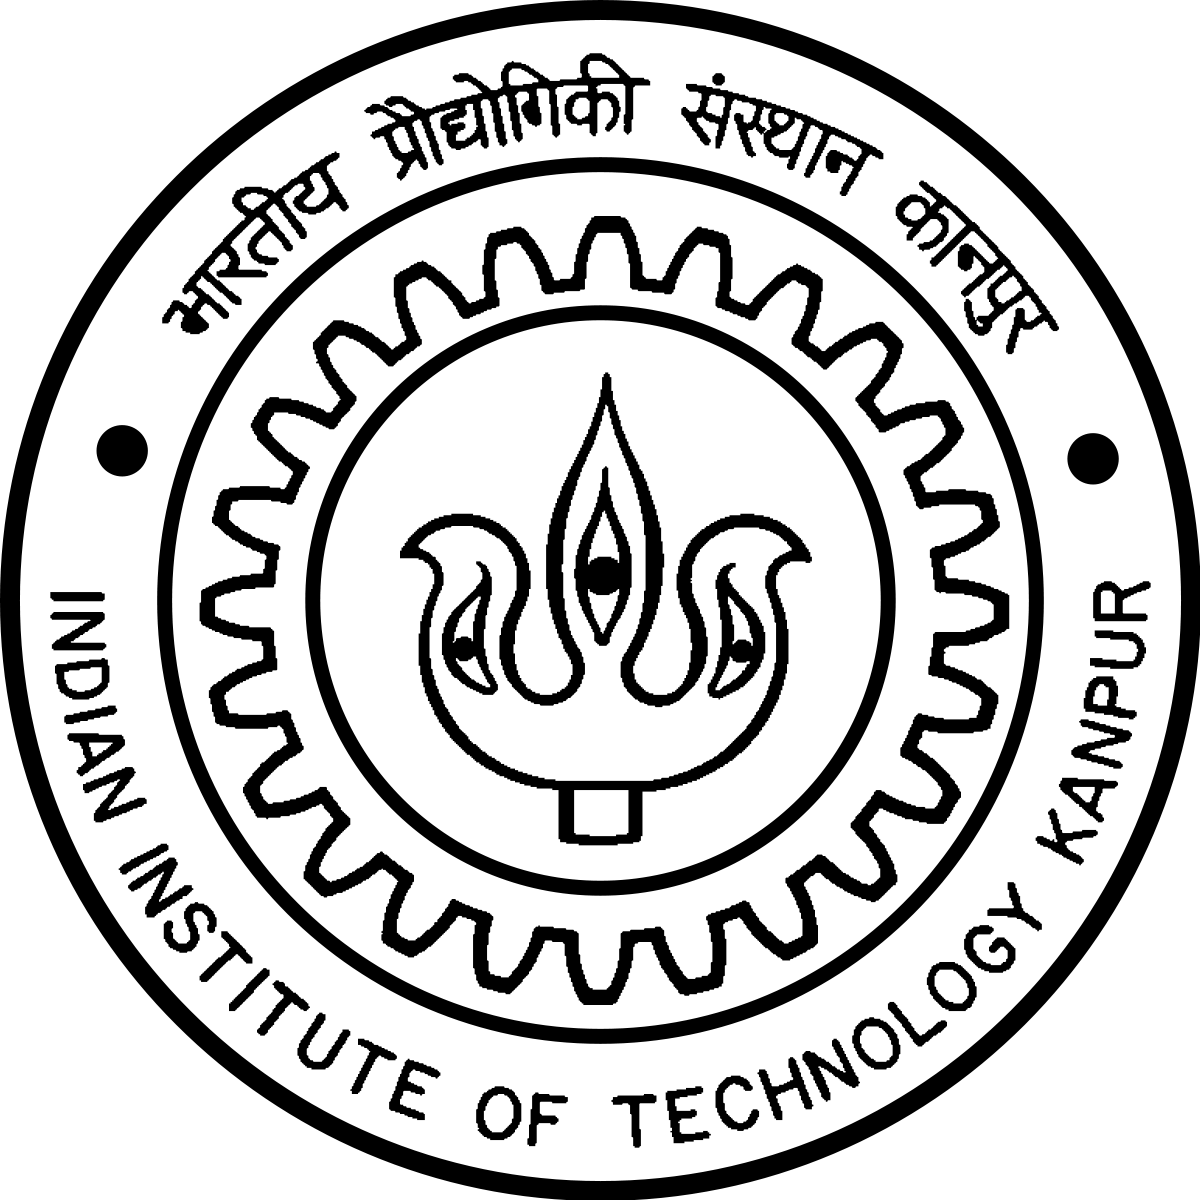
\includegraphics[width=3.2cm]{logo.png}\par
}{%
  \framebox{\parbox[c][2.8cm][c]{2.8cm}{\centering\small\textbf{IIT Kanpur}\\\textbf{Logo}\\(\texttt{logo.png})}}\par
}
\vspace*{1.0cm}
{\LARGE\bfseries \projecttitle\par}
\vspace{1.8cm}
{\Large Aurav Pratap Singh\par}
\vspace{0.25cm}
{\large Roll Number: 230243 \par}
\vspace{1.0cm}
{\large Project Supervisor: Satya Prakash Singh\par}
\vspace{1.9cm}
{\large\bfseries \projectcourse\par}
\vspace{0.7cm}
{\large \department\par}
{\large \institution\par}

\vfill
{\large \today\par}
\vspace*{0.8cm}
\end{titlepage}

% ============================ FRONT MATTER ============================
\pagenumbering{roman}
\setcounter{page}{1}
\tableofcontents
\clearpage
\listoffigures
\clearpage
\listoftables
\clearpage

\chapter*{Abstract}
\addcontentsline{toc}{chapter}{Abstract}
Agricultural commodity prices are reported for particular markets, dates, crops, varieties, and grades. A useful forecasting system should therefore be able to construct a separate chronological price series for the commodity or variety selected by a user, rather than treating all quoted prices as one undifferentiated series. This project develops a general, data-driven framework for forecasting selected mandi prices using an adaptive, gap-aware Kalman filter. The method estimates a hidden price level and a local trend, and updates those estimates whenever a new market quotation becomes available.

The website is designed to let a user select the state, district, market, commodity, variety, and grade, inspect the observed history, and request a short-horizon forecast. The same forecasting procedure can be applied independently to each eligible selected series, provided records for that selection exist in the data source. The supplied dataset used for the numerical case study currently contains wheat quotations at Kanpur (Grain) APMC across 11 varieties. Accordingly, the detailed numerical results in this report are results for the wheat case study; they do not claim that every other commodity has already been empirically validated. On the current file, 870 valid variety-level rows are aggregated into 221 observed date-level prices from 11 November 2025 to 21 September 2026, with 94 calendar dates in the inclusive span having no recorded observation.

For the wheat case study, the first 100 observed prices initialize the filter and the following 121 observations are evaluated sequentially in a walk-forward experiment. The adaptive, gap-aware filter obtains a mean absolute error of approximately Rs.\ 18.87 per quintal, a root mean squared error of Rs.\ 24.34 per quintal, and a mean absolute percentage error of 0.740\%. A previous-price benchmark obtains a MAPE of 0.746\%, so the improvement is modest. The report develops the necessary mathematics from elementary time-series notation, descriptive statistics, random variables, and covariance matrices through state-space modelling, the Kalman gain, adaptive noise scales, uncertainty intervals, and time-ordered evaluation. It also introduces the basic web architecture and separates features implemented in the current CSV-backed prototype from future live-data integration.

\clearpage
\chapter*{Declaration}
\addcontentsline{toc}{chapter}{Declaration}
I hereby declare that this report presents the mathematical and computational work undertaken for the undergraduate project entitled \emph{\projecttitle}. Ideas, equations, methods, and statements taken from published sources are acknowledged through citations and the bibliography. Project-specific numerical results are computed from the mandi price dataset described in this report. The name, roll number, and supervisor fields on the title page are placeholders to be completed before submission.

\vspace{1.2cm}
\noindent Name and Signature: \rule{7cm}{0.4pt}

\vspace{0.8cm}
\noindent Date: \rule{4cm}{0.4pt}

\clearpage
\pagenumbering{arabic}
\setcounter{page}{1}

% ============================== CHAPTER 1 ==============================
\chapter{Introduction}

\section{Motivation}
A time series is a collection of numerical observations ordered by time. Standard treatments emphasize that the time ordering and the way a series is sampled are part of the model, rather than merely formatting details \cite{hamilton1994,hyndman2021}. Examples include daily temperature, hourly electricity demand, monthly inflation, and the price of an agricultural commodity at a wholesale market. In this project, a user selects a market and a commodity or variety, and the forecasting procedure operates on the corresponding price series. The modal price is the market-reported modal quotation for the selected item. The supplied file used for the numerical case study contains wheat varieties, so wheat is used to explain and evaluate the mathematics; the underlying procedure is not specific to wheat.

A direct forecast based only on the latest observation is easy to compute, but it does not explicitly estimate whether prices have been rising or falling. A moving average can smooth short-term fluctuations, but its response is controlled indirectly by the chosen window. A state-space model offers another representation: it separates the observed price from a hidden state describing the evolving price level and trend. The Kalman filter updates this hidden state recursively as new observations arrive \cite{kalman1960,welch2006,durbin2012}.

The choice is practical as well as mathematical. The method is lightweight, updates without refitting a large model from scratch, and can naturally represent uncertainty in its current state estimate. The dataset also has missing calendar dates. Rather than inventing a price on each missing day, the transition equation can explicitly use the number of elapsed days between two observed market dates.

\section{Project objectives}
The project has six main objectives:
\begin{enumerate}
  \item design a reusable workflow that can construct a date-level price series for a selected agricultural commodity, variety, grade, and market;
  \item introduce the basic concepts of time-series analysis, random variables, noise, matrices, and state-space models needed to formulate a forecasting problem;
  \item derive and implement the prediction and correction equations of a Kalman filter with latent price level and trend;
  \item make the filter adaptive to changing short-run variation and aware of gaps between observation dates;
  \item evaluate sequential forecasts with standard error measures and compare them against a simple previous-price benchmark;
  \item present historical prices and forecasts through a simple website that allows users to select the available market and commodity dimensions.
\end{enumerate}

\section{Scope and what is not claimed}
The forecast is univariate for each selected series: it uses that series' historical target prices, not weather, wholesale demand, government minimum support price announcements, fuel prices, or other explanatory variables. It is not a seasonal ARIMA, an LSTM network, or a causal model of agricultural markets. The Kalman filter estimates a smooth latent level and a local trend under a specified state-space model. Its noise parameters are adjusted by transparent heuristic recursions rather than estimated by a full maximum-likelihood procedure. Separate commodities must be modelled separately; prices of different commodities or incompatible units must not be averaged together.

The website is intended to support selection among the market and commodity options present in its data. The supplied CSV snapshot used for this report contains wheat only, with multiple wheat varieties, so the reported numerical accuracy measures are for that case study. The current prototype reads an offline CSV file; it does not yet connect to a live market-data API, automated scraper, scheduled ingestion job, database, or production monitoring service. The website architecture and data flow are described in Chapter~7.

\section{Organization of the report}
Chapter 2 introduces the mathematical and statistical preliminaries. Chapter 3 describes the dataset and construction of the target series. Chapter 4 develops the local linear-trend state-space model. Chapter 5 derives the Kalman filter and explains the adaptive and gap-aware modifications. Chapter 6 gives the evaluation design and results. Chapter 7 describes the computational implementation and website architecture, then discusses assumptions and limitations. Chapter 8 summarizes the work and outlines future extensions.

% ============================== CHAPTER 2 ==============================
\chapter{Preliminaries}
This chapter introduces the language and notation used throughout the project. The aim is not to give a complete course in time-series analysis, but to establish each concept needed to understand the model and its implementation.

\section{Time series and the time index}
\begin{definition}[Time series]
A time series is a sequence of observations indexed by time. In discrete notation it is written as
\[
  y_1,y_2,\ldots,y_n,
\]
where $y_t$ is the value recorded at observation index $t$.
\end{definition}

The subscript $t$ is often called a time index. It is important to distinguish the observation index from calendar time. If a market reports a price on Monday and then on Wednesday, those are consecutive observations, but two calendar days have elapsed. We denote the calendar date of observation $t$ by $d_t$ and the elapsed time between observations by
\[
  \Delta_t = \max\{(d_t-d_{t-1})\text{ measured in days},1\}.
\]
This report uses $t$ to identify the observation in the sorted series and $\Delta_t$ to describe the actual time gap. When the dates are consecutive, $\Delta_t=1$.

\section{Components of a time series}
A time series may contain several kinds of structure.
\begin{itemize}
  \item \textbf{Level:} the current baseline around which observations vary.
  \item \textbf{Trend:} a persistent local tendency for the series to rise or fall.
  \item \textbf{Seasonality:} a pattern that repeats at a known period, such as a weekly or yearly pattern.
  \item \textbf{Cycle:} a longer or less regular pattern of expansion and contraction.
  \item \textbf{Irregular variation:} short-term changes not explained by the explicitly modelled components.
\end{itemize}

A generic conceptual decomposition is
\begin{equation}
  y_t = \ell_t + s_t + r_t,
  \label{eq:decomposition}
\end{equation}
where $\ell_t$ is a level component, $s_t$ represents a seasonal component, and $r_t$ collects remaining variation. Equation~\eqref{eq:decomposition} is a general way to think about a series; the model used in this project does not contain an explicit seasonal state. Instead, it models a changing level and trend, with the observation and process noise terms accounting for unexplained variation.

\section{Lagged observations and first differences}
A lag is a past observation. For example, $y_{t-1}$ is the previous observed value. The first difference is
\begin{equation}
  \Delta y_t = y_t-y_{t-1}.
  \label{eq:firstdiff}
\end{equation}
It records the absolute change between consecutive observed entries. If prices are measured in rupees per quintal, the difference has the same unit. The difference series is useful in this project for estimating the initial variability and for obtaining an initial estimate of the trend. It is not itself the target of a separate forecasting model.

For a regularly sampled series, a first difference can be viewed as a one-period change. If the calendar interval varies, $\Delta y_t$ spans $\Delta_t$ days. A per-day change could instead be formed as $(y_t-y_{t-1})/\Delta_t$. The current implementation uses raw differences for its variance heuristics, while the state-transition matrix explicitly accounts for elapsed calendar time. This distinction is discussed again in Chapter~7.

\section{Descriptive statistics used by the model}
\subsection{Arithmetic mean and median}
For $n$ numerical observations, the arithmetic mean is
\begin{equation}
  \bar y = \frac{1}{n}\sum_{i=1}^{n} y_i.
\end{equation}
The median is the middle observation after sorting, or the average of the two middle observations when $n$ is even. The mean is sensitive to unusually large or small observations; the median is more robust to extreme values. In this project, the mean is used for fallback aggregation when all arrival weights sum to zero, and the median of recent first differences initializes the trend. The median makes the initial trend less sensitive to a single large difference than an ordinary mean would be.

\subsection{Sample variance}
The sample variance measures dispersion around the sample mean:
\begin{equation}
  s^2 = \frac{1}{n-1}\sum_{i=1}^{n}(z_i-\bar z)^2,
  \qquad \bar z=\frac{1}{n}\sum_{i=1}^{n}z_i.
  \label{eq:samplevar}
\end{equation}
The square root $s$ is the sample standard deviation, which has the same units as the values. Variance has squared units. For example, if $z_i$ is a price difference in Rs./quintal, $s^2$ is measured in $(\text{Rs./quintal})^2$. The implementation estimates an initial variance from the first differences in the first 100 observations and later recomputes a rolling variance using recent differences.

\subsection{Arrival-weighted mean}
If observations have different weights, the weighted mean is
\begin{equation}
  \bar p_w = \frac{\sum_{j=1}^{m} a_jp_j}{\sum_{j=1}^{m}a_j},
  \qquad \sum_{j=1}^{m}a_j>0,
  \label{eq:weightedmean}
\end{equation}
where $p_j$ is a quoted modal price and $a_j$ is the corresponding arrival quantity. The weighted mean gives greater influence to prices associated with larger recorded arrivals. The aggregation is meaningful only when prices being combined refer to the same commodity, date, market context, and compatible units. In the general system, the date-level aggregation is performed after applying the user's selection, and only records within that selected price series are combined. The supplied numerical case study applies this calculation to the wheat records in the provided market report.

\section{Random variables and stochastic processes}
A random variable represents an uncertain numerical outcome. Its expectation, written $\E[X]$, is its probability-weighted mean, while its variance is
\begin{equation}
  \Var(X)=\E\left[(X-\E[X])^2\right].
\end{equation}
A stochastic process $\{X_t\}$ is a sequence of random variables indexed by time. A state-space model treats the true or latent market state as a stochastic process and the reported market price as an observation generated from that state.

\subsection{Noise and the zero-mean assumption}
The model distinguishes two kinds of noise. \emph{Process noise} represents random changes in the hidden level and trend that the transition equation does not predict exactly. \emph{Observation noise} represents the discrepancy between the latent price level and the reported price. Their mathematical roles are different, even though both are uncertain quantities.

The basic model assumes zero-mean noise:
\[
  \E[w_t]=0,\qquad \E[v_t]=0.
\]
A zero mean says that the noise is not systematically positive or negative in expectation. In a standard linear-Gaussian Kalman filter, the noises are also assumed to be Gaussian and uncorrelated with one another and with the prior state-estimation error. The project uses the Kalman recursions and Gaussian-style uncertainty calculations, but the market data are not proven to be exactly Gaussian. The assumptions are modelling approximations, not claims about every market shock.

\subsection{Gaussian distribution}
A scalar random variable $X$ is Gaussian with mean $\mu$ and variance $\sigma^2$ if its density is
\[
  f_X(x)=\frac{1}{\sqrt{2\pi\sigma^2}}
  \exp\left(-\frac{(x-\mu)^2}{2\sigma^2}\right).
\]
A Gaussian model is convenient because linear transformations of jointly Gaussian vectors remain Gaussian, and a conditional distribution is summarized by its mean and covariance. These properties lead to the standard Kalman filter equations \cite{kalman1960,welch2006}. In empirical forecasting, intervals based on this assumption should be checked against observed forecast errors.

\section{Vectors, matrices, and covariance matrices}
The state contains two numbers, so it is represented as a column vector. For vectors $x\in\R^n$ and matrices $A\in\R^{m\times n}$, matrix multiplication $Ax$ forms linear combinations of the entries of $x$. The transpose $A\trans$ swaps rows and columns.

For a random vector $X$, the covariance matrix is
\begin{equation}
  \Cov(X)=\E\left[(X-\E[X])(X-\E[X])\trans\right].
\end{equation}
The diagonal entries are component variances and the off-diagonal entries are covariances between components. A covariance matrix is symmetric and positive semidefinite: for every vector $u$, $u\trans\Cov(X)u\geq 0$. In the Kalman filter, the matrix $P_t$ stores the uncertainty in the estimated state and the matrix $Q_t$ stores process-noise covariance. The observation-noise covariance $R_t$ is scalar in this one-observation model.

For a deterministic matrix $A$ and a random vector with covariance $P$, covariance transforms according to
\begin{equation}
  \Cov(AX)=A\Cov(X)A\trans.
  \label{eq:covtransform}
\end{equation}
Adding independent noise with covariance $Q$ adds $Q$ to the covariance in~\eqref{eq:covtransform}. This is the origin of the Kalman prediction covariance equation.

\section{Forecasting, filtering, and smoothing}
These related tasks should not be confused.
\begin{itemize}
  \item \textbf{Forecasting} estimates a future quantity using observations available now.
  \item \textbf{Filtering} estimates the current hidden state using observations up to and including the current time.
  \item \textbf{Smoothing} estimates a past hidden state using observations from both before and after that time.
\end{itemize}
The project uses filtering recursively to update the state and forecasting to predict before the next observation arrives. It does not use a backward smoothing pass. The key rule in evaluation is temporal order: the prediction for date $t$ is calculated before the actual price at date $t$ is used to update the filter.

% ============================== CHAPTER 3 ==============================
\chapter{Dataset and Construction of the Target Series}

\section{Description of the data}
The supplied project dataset \cite{projectdata} is named \texttt{Daily Price Arrival Report-07-11-2025 to 21-09-2026 for Uttar Pradesh.csv}. Its schema contains state, district, market, commodity group, commodity, variety, grade, minimum price, maximum price, modal price, price unit, arrival quantity, arrival unit, and arrival date. This schema is appropriate for a system that lets a user select among the commodity and market dimensions represented in a data source. In the particular CSV supplied for the numerical case study, the records are for wheat varieties at Kanpur (Grain) APMC in Kanpur district, Uttar Pradesh; the present file does not contain other commodity names. The file includes a title row before the field-name row, so the data-processing step removes the title and uses the second row as the column header.

After converting price and arrival columns to numeric values, parsing dates, clipping negative arrivals to zero, and removing rows without a valid date, modal price, or arrival quantity, 870 rows remain. Those rows map to 221 distinct recorded dates between 11 November 2025 and 21 September 2026. The file name advertises an earlier beginning date, but the first valid price date in the rows is 11 November 2025; the analysis uses the actual valid records rather than inventing earlier values.

\begin{table}[H]
\centering
\caption{Profile of the cleaned project data}
\label{tab:datasetprofile}
\begin{tabular}{@{}ll@{}}
\toprule
Quantity & Value \\
\midrule
Valid variety-level rows & 870 \\
Observed date-level prices & 221 \\
First observed date & 11 November 2025 \\
Last observed date & 21 September 2026 \\
Distinct varieties in source & 11 \\
Districts represented & 1 (Kanpur) \\
Markets represented & 1 (Kanpur (Grain) APMC) \\
Commodity in this case study & Wheat \\
Price unit & Rs. per quintal \\
Arrival quantity unit & Metric tonnes \\
Calendar dates without a record within the observed span & 94 \\
\bottomrule
\end{tabular}
\end{table}

\section{Data cleaning}
Let a raw row be indexed by $j$ and let $d_j$ be its arrival date. The preprocessing follows these steps:
\begin{enumerate}
  \item remove the descriptive title line and parse the field-name row;
  \item convert commas in numeric strings to standard numeric values for minimum, maximum, and modal price and arrival quantity;
  \item parse dates using day-first interpretation;
  \item replace invalid numeric entries with missing values and exclude rows without a usable date, modal price, or arrival quantity;
  \item clip negative arrival quantities to zero, since negative physical arrival is not meaningful as a weighting amount;
  \item group remaining rows by arrival date, compute the daily weighted modal price, sum daily arrivals, and sort the date-level observations chronologically.
\end{enumerate}

The preprocessing reduces the data from individual variety-level rows to one target price per observed date. It does not create artificial observations on days absent from the file. This choice preserves the distinction between a missing market record and an actual market quote.

\section{Definition of the daily target price}
Suppose that on date $d_t$ there are $m_t$ valid variety-level records. Write $p_{t,j}$ for the modal price in row $j$ and $a_{t,j}$ for its nonnegative arrival quantity. The target used in the main experiment is
\begin{equation}
  y_t=\begin{cases}
  \displaystyle\frac{\sum_{j=1}^{m_t}a_{t,j}p_{t,j}}
  {\sum_{j=1}^{m_t}a_{t,j}}, & \text{if }\sum_{j=1}^{m_t}a_{t,j}>0,\\[1.2em]
  \displaystyle\frac{1}{m_t}\sum_{j=1}^{m_t}p_{t,j}, & \text{if all arrival weights sum to zero.}
  \end{cases}
  \label{eq:dailyprice}
\end{equation}
Equation~\eqref{eq:dailyprice} is applied separately on each recorded date. The arrival-weighted mean represents the day's mix of reported varieties in proportion to their recorded arrival quantity. A change in the daily aggregate can arise from a change in the price of a given variety, a change in the quantities arriving, a change in the varieties reported, or a combination of these factors. Consequently, the aggregate is a useful market-level indicator but is not identical to a single fixed variety's price.

\begin{example}[A simple weighted average]
Suppose two variety records have modal prices Rs.\ 2,500 and Rs.\ 2,600 per quintal, with arrivals of 10 and 30 metric tonnes. Then the weighted mean is
\[
 \frac{10(2500)+30(2600)}{10+30}=\Rs.\ 2,575\text{ per quintal}.
\]
The second quotation receives more weight because its recorded arrival quantity is larger. This example illustrates the arithmetic; it is not a row from the data file.
\end{example}

\section{Missing calendar dates and irregular time steps}
The observed dates occupy a period of 315 calendar days when both endpoints are counted, but only 221 date-level prices are present. Thus, 94 dates in this inclusive span do not have an observed price. Missing observations are not automatically evidence that the price was constant or that the market was closed; they indicate only that the provided report contains no usable observation for those dates.

For consecutive observations, the elapsed time is computed as
\begin{equation}
  \Delta_t=\max\{(d_t-d_{t-1})\text{ in calendar days},1\}.
  \label{eq:dt}
\end{equation}
The model propagates the state using this gap rather than pretending that every row is exactly one day after the previous row. This is called gap-aware or irregular-time-step handling. Forecast errors in the test segment are calculated at the dates with actual records. Therefore, the backtest is one-observation-ahead; when a calendar gap occurs, the forecast is propagated over that many days and compared with the next recorded price.

\section{Exploratory view of the series}
Figure~\ref{fig:series} displays the resulting daily target series for the wheat case study. The observed aggregate price varies between approximately Rs.\ 2,300 and Rs.\ 2,701 per quintal. Its sample mean is Rs.\ 2,483.41, its median is Rs.\ 2,462.32, and its sample standard deviation is approximately Rs.\ 101.39 per quintal. These summary statistics describe the observed target series, not a probability law that the future price must follow.

\begin{figure}[H]
\centering
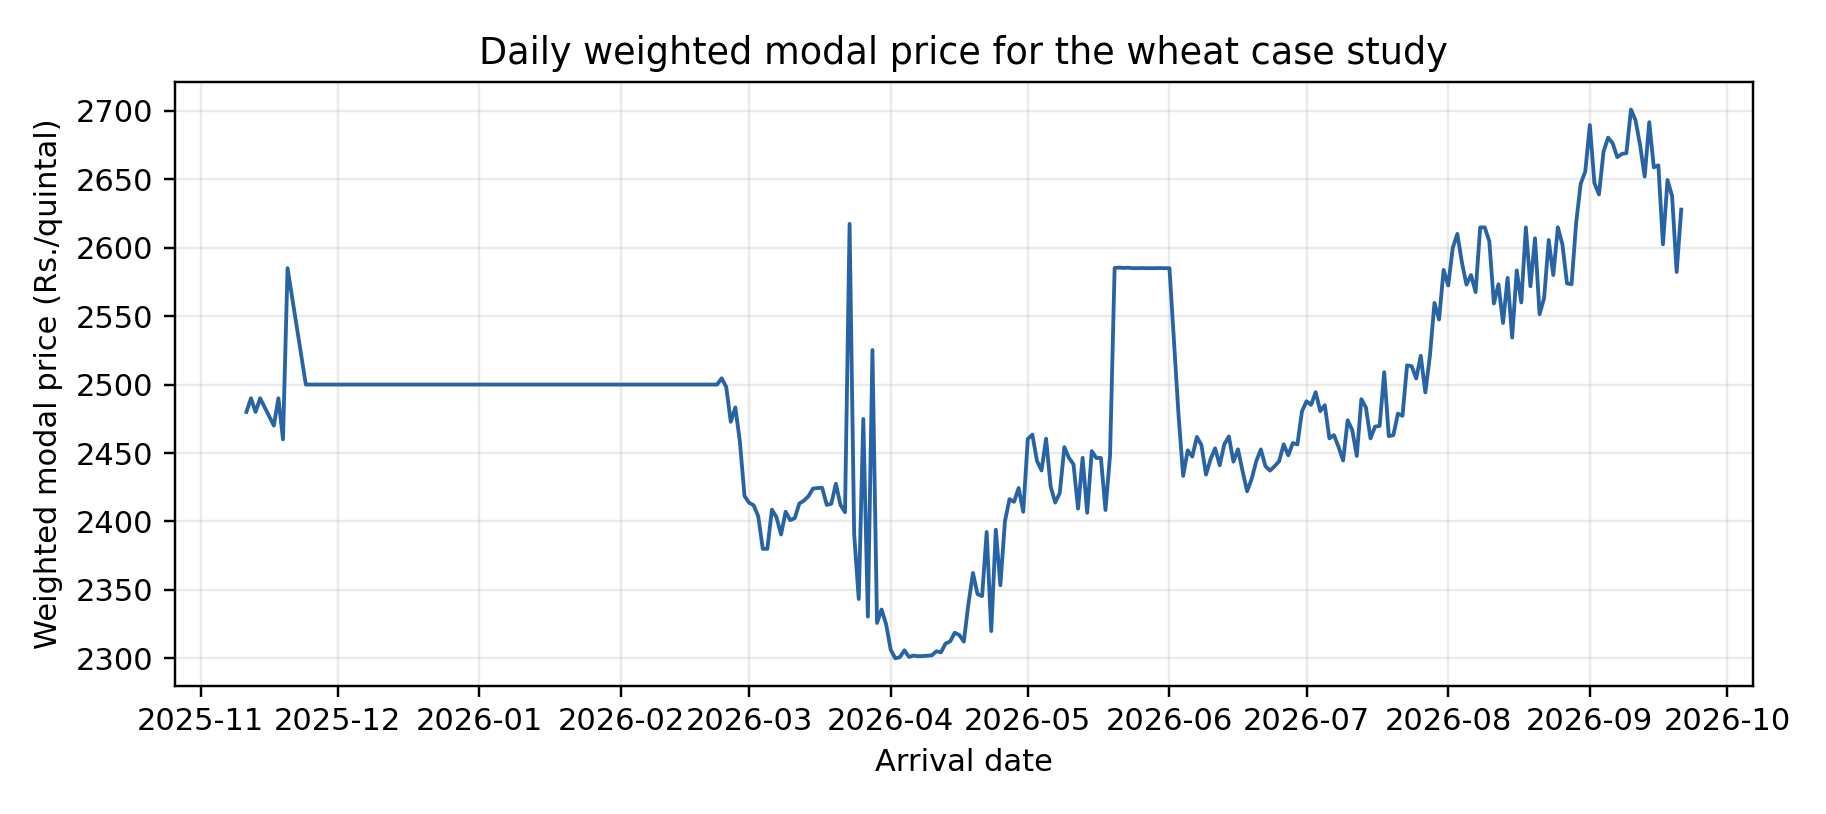
\includegraphics[width=0.96\textwidth]{01_daily_price_series.png}
\caption{Daily arrival-weighted modal price for the wheat case study, after grouping selected records by arrival date. Gaps in the source have not been filled with fabricated price observations.}
\label{fig:series}
\end{figure}

\section{Why aggregation choices matter}
A time series model requires a precisely defined target. If the objective is to forecast one variety such as Dara, then other varieties should be filtered out before date-level aggregation. If the objective is a mixed all-variety indicator, then a weighted daily mean such as~\eqref{eq:dailyprice} is appropriate. These targets answer different questions and can produce different scores. The main numerical results below refer to the weighted all-variety target. They should not be mixed with results from the separate Dara-only series.

% ============================== CHAPTER 4 ==============================
\chapter{The Local Linear-Trend State-Space Model}

\section{Observed quantity and hidden state}
The value $y_t$ is observed, but the underlying state used by the filter is not directly observed. In this project the hidden state is a two-dimensional vector
\begin{equation}
  x_t=\begin{bmatrix}\ell_t\\ b_t\end{bmatrix},
  \label{eq:state}
\end{equation}
where $\ell_t$ denotes the latent price level and $b_t$ denotes the local trend, interpreted as a change in price per day under the model's daily transition convention. The level is the model's estimate of the current underlying price; the trend describes the direction and approximate rate at which that level is moving.

The word \emph{latent} does not mean that the level can be observed separately in the data. It means that it is a model-defined hidden quantity inferred from observed prices. The actual market price contains both the latent level and observation noise. The two-state representation is more flexible than using only a level because it can extrapolate recent movement instead of always assuming that the next price equals the latest level.

\section{From level and trend to a state transition}
If the trend were constant for one day and there were no random disturbances, the local linear model would be
\[
  \ell_t=\ell_{t-1}+b_{t-1},\qquad b_t=b_{t-1}.
\]
For an elapsed interval of $\Delta_t$ days, the corresponding deterministic relation becomes
\[
  \ell_t=\ell_{t-1}+\Delta_tb_{t-1},\qquad b_t=b_{t-1}.
\]
A real market does not follow this deterministic relation exactly, so we add a process disturbance $w_t$. In vector form,
\begin{equation}
  x_t=F_t x_{t-1}+w_t,
  \qquad
  F_t=\begin{bmatrix}1&\Delta_t\\0&1\end{bmatrix}.
  \label{eq:transition}
\end{equation}
Writing out the two coordinates gives
\begin{align}
  \ell_t &= \ell_{t-1}+\Delta_t b_{t-1}+w_{\ell,t},\\
  b_t &= b_{t-1}+w_{b,t}.
\end{align}
The transition matrix $F_t$ is time-dependent through $\Delta_t$. If no days have elapsed beyond the usual one-day interval, it reduces to $\begin{bmatrix}1&1\\0&1\end{bmatrix}$.

\section{The observation equation}
Only the level, rather than the trend directly, is observed. The measurement equation is
\begin{equation}
  y_t=Hx_t+v_t,
  \qquad H=\begin{bmatrix}1&0\end{bmatrix},
  \label{eq:observation}
\end{equation}
where $v_t$ is the observation noise. Multiplying out $Hx_t$ gives $Hx_t=\ell_t$, so the equation states $y_t=\ell_t+v_t$. A high observation does not automatically mean that the true level jumped by the full amount: the filter uses its uncertainty and the observation-noise estimate to decide how strongly to react.

\section{Process noise and observation noise}
The process noise $w_t$ is modelled to have mean zero and covariance $Q_t$:
\begin{equation}
  \E[w_t]=0,\qquad \Cov(w_t)=Q_t
  =\begin{bmatrix}q_{\ell,t}&0\\0&q_{b,t}\end{bmatrix}.
  \label{eq:Q}
\end{equation}
Here $q_{\ell,t}$ controls uncertainty associated with movement of the level, while $q_{b,t}$ controls uncertainty about changes in trend. The off-diagonal entries are set to zero by the implementation; thus, it does not explicitly model correlation between the two process-noise components.

The observation noise $v_t$ is scalar with
\begin{equation}
  \E[v_t]=0,\qquad \Var(v_t)=R_t.
  \label{eq:R}
\end{equation}
A larger $R_t$ tells the filter to treat the observed price as relatively noisy. A larger $Q_t$ tells it that the underlying state may change more unpredictably. These parameters have different conceptual functions: $Q_t$ describes uncertainty in the state evolution, whereas $R_t$ describes uncertainty in the measurement equation.

\section{State estimate and error covariance}
At each time, the filter stores an estimate of the state and an uncertainty matrix. Let
\[
  \hatt{x}_{t|t}=\E[x_t\given y_1,\ldots,y_t]
\]
under the linear-Gaussian model. The notation $t|t$ means that observations through $t$ have been used. The covariance of the state-estimation error is
\begin{equation}
  P_{t|t}=\E\left[(x_t-\hatt{x}_{t|t})(x_t-\hatt{x}_{t|t})\trans\right].
\end{equation}
Before the new observation at $t$ is used, the corresponding quantities are written $\hatt{x}_{t|t-1}$ and $P_{t|t-1}$. This notation distinguishes the \emph{prior/predicted} state from the \emph{posterior/updated} state.

\section{Interpretation of the assumptions}
The state-space model assumes that the next hidden state is a linear transformation of the previous hidden state plus a random disturbance, and the observed price is a linear function of the current state plus measurement noise. The Kalman recursion is exact for linear models with Gaussian disturbances and known noise covariances. In this project the model is linear, but the noise covariances are adapted by heuristics and the empirical distribution of market shocks is not known to be Gaussian. It is therefore most accurate to describe the method as an adaptive Kalman filter motivated by the standard linear-Gaussian theory.

% ============================== CHAPTER 5 ==============================
\chapter{The Adaptive, Gap-Aware Kalman Filter}

\section{The central idea}
The Kalman filter repeatedly performs two operations. First, it predicts what the hidden state and the next observation should be using the previous updated state. Second, when the next price becomes available, it uses the prediction error to correct the hidden state. The filter does not need to store all past observations in order to perform each update; it carries forward the state estimate and its covariance. This recursive property is one reason Kalman filtering is useful in online estimation \cite{kalman1960,welch2006}.

A useful conceptual diagram is shown in Figure~\ref{fig:workflow}. The prediction occurs before the new price is incorporated; this ordering is essential both for a realistic forecasting process and for a leakage-free evaluation.

\begin{figure}[H]
\centering
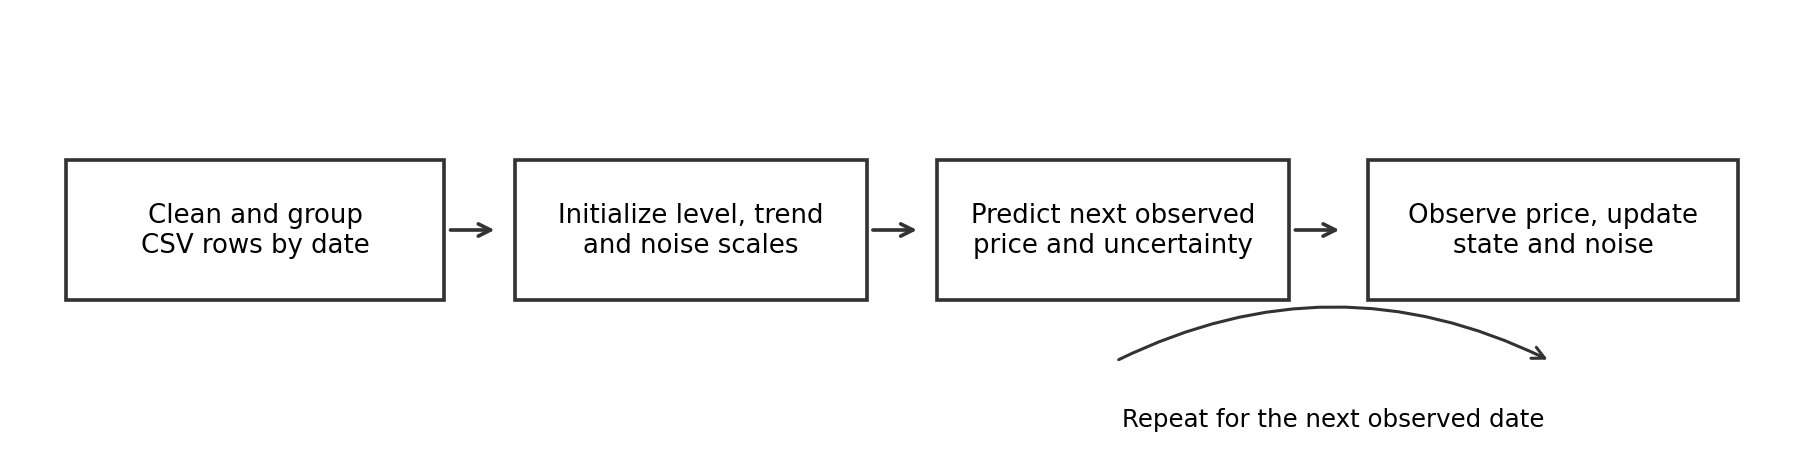
\includegraphics[width=0.98\textwidth]{05_workflow.png}
\caption{High-level workflow of the data aggregation and recursive Kalman update.}
\label{fig:workflow}
\end{figure}

\section{Initialization}
A recursive algorithm needs a starting state and starting uncertainty. Let $n_{\mathrm{train}}=100$. Define the first-difference sequence over the initial segment by $d_i=y_i-y_{i-1}$. The initial variance scale is
\begin{equation}
  s_0^2=\max\left\{\frac{1}{n_{\mathrm{train}}-2}
  \sum_{i=2}^{n_{\mathrm{train}}}(d_i-\bar d)^2,10^{-6}\right\},
  \label{eq:initvar}
\end{equation}
where the code calculates the sample variance of the first differences and floors it at $10^{-6}$ to prevent degenerate numerical values. The lower bound is a numerical safeguard; it is not a statement that the market variance is known to be at least this physical amount.

The initial state is
\begin{equation}
  \hatt{x}_{n_{\mathrm{train}}|n_{\mathrm{train}}}
  =\begin{bmatrix}y_{n_{\mathrm{train}}}\\
  \operatorname{median}(d_{n_{\mathrm{train}}-8},\ldots,d_{n_{\mathrm{train}}})\end{bmatrix},
  \label{eq:initstate}
\end{equation}
with the implementation's indexing convention that the initial level is the 100th observed price and the initial trend is the median of the nine first differences among the final ten training prices. The initial state covariance is
\begin{equation}
  P_0=s_0^2I_2,
  \label{eq:initP}
\end{equation}
where $I_2$ is the $2\times2$ identity matrix. This assigns the same initial numerical variance scale to the level and trend coordinates for simplicity. Because level and trend have different physical units, this is a heuristic initialization and not a unit-invariant statistical estimate.

The initial process and observation noise values are
\begin{equation}
  Q_0=\begin{bmatrix}0.20s_0^2&0\\0&0.02s_0^2\end{bmatrix},
  \qquad R_0=\max\{0.15s_0^2,10^{-6}\}.
  \label{eq:initQR}
\end{equation}
The relative factors $0.20$, $0.02$, and $0.15$ are implementation choices. They are not universal constants of Kalman filtering and would be candidates for calibration in a more systematic model-selection study.

\section{Prediction of the state}
Assume the updated state at the preceding observation is $\hatt{x}_{t-1|t-1}$ with covariance $P_{t-1|t-1}$. Given the transition matrix $F_t$ from~\eqref{eq:transition}, the predicted state is
\begin{equation}
  \hatt{x}_{t|t-1}=F_t\hatt{x}_{t-1|t-1}.
  \label{eq:predstate}
\end{equation}
For this project's two state variables, the equation is
\[
  \begin{bmatrix}\hatt{\ell}_{t|t-1}\\\hatt{b}_{t|t-1}\end{bmatrix}
  =\begin{bmatrix}1&\Delta_t\\0&1\end{bmatrix}
  \begin{bmatrix}\hatt{\ell}_{t-1|t-1}\\\hatt{b}_{t-1|t-1}\end{bmatrix},
\]
which gives
\begin{align}
  \hatt{\ell}_{t|t-1}&=\hatt{\ell}_{t-1|t-1}+\Delta_t\hatt{b}_{t-1|t-1},\\
  \hatt{b}_{t|t-1}&=\hatt{b}_{t-1|t-1}.
\end{align}
The predicted observation is obtained from the observation equation:
\begin{equation}
  \hatt{y}_{t|t-1}=H\hatt{x}_{t|t-1}=\hatt{\ell}_{t|t-1}.
  \label{eq:predobs}
\end{equation}
This is the value recorded as the forecast before the actual price $y_t$ is used in the update.

\section{Prediction of state uncertainty}
The state prediction is uncertain even if the previous state estimate is known. Let $e_{t-1}=x_{t-1}-\hatt{x}_{t-1|t-1}$ be the previous estimation error. Using $x_t=F_tx_{t-1}+w_t$ and the predicted mean in~\eqref{eq:predstate}, the predicted error is
\[
  x_t-\hatt{x}_{t|t-1}=F_te_{t-1}+w_t.
\]
If the previous error and current process noise are uncorrelated, the cross-covariance terms vanish. Applying the covariance transformation rule~\eqref{eq:covtransform} gives
\begin{equation}
  P_{t|t-1}=F_tP_{t-1|t-1}F_t\trans+Q_t.
  \label{eq:predcovstandard}
\end{equation}
The gap-aware implementation uses the approximation
\begin{equation}
  P_{t|t-1}=F_tP_{t-1|t-1}F_t\trans+\Delta_tQ_t.
  \label{eq:predcovgap}
\end{equation}
Thus uncertainty is propagated through the transition matrix and augmented in proportion to the elapsed number of days. Equation~\eqref{eq:predcovstandard} is the familiar discrete-time Kalman form; Equation~\eqref{eq:predcovgap} describes the actual gap-scaling convention implemented in this project. It should be regarded as a practical approximation rather than the unique continuous-time discretization of every possible stochastic trend model.

\section{Innovation: the prediction error}
Once the market price at date $t$ is observed, the innovation is defined as
\begin{equation}
  e_t=y_t-H\hatt{x}_{t|t-1}=y_t-\hatt{y}_{t|t-1}.
  \label{eq:innovation}
\end{equation}
An innovation is positive when the observed price is higher than predicted and negative when it is lower. A value close to zero indicates that the prediction was close to the observation. The term \emph{innovation} is used because it is the new information in the observation relative to the forecast made from past information.

The predicted innovation variance is
\begin{equation}
  S_t=HP_{t|t-1}H\trans+R_t.
  \label{eq:S}
\end{equation}
Since $H=[1\quad 0]$, this reduces to
\begin{equation}
  S_t=(P_{t|t-1})_{11}+R_t.
  \label{eq:Sscalar}
\end{equation}
The first term is uncertainty about the predicted level; the second is observation-noise variance. In this one-dimensional observation setting, $S_t$ is a scalar.

\section{Kalman gain and its interpretation}
The Kalman gain tells the filter how much of the innovation should be used to correct each state coordinate. It is
\begin{equation}
  K_t=P_{t|t-1}H\trans S_t^{-1}.
  \label{eq:gain}
\end{equation}
Because $P_{t|t-1}$ is $2\times2$, $H\trans$ is $2\times1$, and $S_t^{-1}$ is scalar, $K_t$ is a $2\times1$ vector. The two entries control the corrections to the level and trend respectively.

For intuition, consider the scalar version in which the only unknown is a level. If the prior estimate has variance $P^-$ and the measurement noise has variance $R$, the gain becomes
\[
  K=\frac{P^-}{P^-+R}.
\]
If $P^-$ is large relative to $R$, the prior estimate is uncertain while the measurement is comparatively reliable, so the gain is large and the observation receives more weight. If $R$ is large relative to $P^-$, the observation is regarded as noisy, so the gain is smaller. In the two-state model this idea is expressed through the covariance between each state coordinate and the observed level.

\subsection{Why this gain is a minimum-variance linear update}
Consider a candidate update $\hatt{x}_{t|t}=\hatt{x}_{t|t-1}+K_te_t$. Let $u_t=x_t-\hatt{x}_{t|t-1}$ be the prior state error, so that the innovation can be written $e_t=Hu_t+v_t$. The posterior error then satisfies
\[
  x_t-\hatt{x}_{t|t}=(I-K_tH)u_t-K_tv_t.
\]
Under the standard uncorrelated-error assumptions, its covariance for an arbitrary gain $K$ is
\begin{equation}
  P(K)=(I-KH)P^-(I-KH)\trans+KRK\trans.
  \label{eq:joseph}
\end{equation}
Minimizing the expected squared Euclidean estimation error is equivalent to minimizing $\tr(P(K))$. Differentiating this quadratic expression with respect to $K$ and setting the derivative to zero gives
\[
  K(HP^-H\trans+R)=P^-H\trans.
\]
When the scalar innovation variance $S=HP^-H\trans+R$ is positive, it follows that
\[
  K=P^-H\trans S^{-1},
\]
which is Equation~\eqref{eq:gain}. This derivation explains the central role of the gain: among linear corrections of this form, it balances prior-state uncertainty against measurement uncertainty.

\section{State correction}
After observing $y_t$, the state is corrected using the innovation:
\begin{equation}
  \hatt{x}_{t|t}=\hatt{x}_{t|t-1}+K_te_t.
  \label{eq:update}
\end{equation}
For the two coordinates,
\begin{align}
  \hatt{\ell}_{t|t}&=\hatt{\ell}_{t|t-1}+K_{\ell,t}e_t,\\
  \hatt{b}_{t|t}&=\hatt{b}_{t|t-1}+K_{b,t}e_t.
\end{align}
Thus, an unexpected upward observation can raise the estimated level and can also alter the estimated trend. The gain vector determines how this surprise is distributed between the components.

\section{Covariance correction}
The posterior state covariance has the simplified form
\begin{equation}
  P_{t|t}=(I-K_tH)P_{t|t-1}.
  \label{eq:covupdate}
\end{equation}
A numerically more robust equivalent under the Kalman assumptions is the Joseph form in~\eqref{eq:joseph} with the gain chosen by~\eqref{eq:gain}. The project implementation uses the simplified update and then replaces the matrix by the average of itself and its transpose:
\[
  P\leftarrow\frac{P+P\trans}{2}.
\]
This symmetrization counters small floating-point asymmetries. It does not substitute for checking positive semidefiniteness, and a more numerically demanding implementation could use the Joseph form directly.

\section{Adaptive observation-noise variance}
In a fixed-noise filter, $R_t$ would remain constant. Here it is updated after each observation using the innovation:
\begin{equation}
  R_{t+1}=0.85R_t+0.15\max\{e_t^2,0.05s_0^2\}.
  \label{eq:adaptiveR}
\end{equation}
This is an exponentially weighted moving average (EWMA)-style recursion. In the general form
\[
  z_{t+1}=(1-\alpha)z_t+\alpha u_t,
\]
the new value $u_t$ receives weight $\alpha$ and the previous estimate receives weight $1-\alpha$. Here $\alpha=0.15$, and the signal is the squared innovation with a small variance floor. A large recent prediction error tends to increase the estimated observation noise, reducing the weight placed on future observations, all else being equal. Smaller squared errors decrease $R_t$ gradually, but the floor prevents it from decaying without bound.

The recursion is adaptive but heuristic. The innovation also contains process-model error and trend misspecification; it is not a pure measurement-noise sample. Therefore, $R_t$ should be interpreted as an effective error scale that includes imperfections not otherwise captured by the model, rather than a direct measurement of physical reporting error.

\section{Adaptive process-noise covariance}
After the filter has processed a few test observations, the implementation estimates recent variation using a rolling window of at most 21 observed prices (at most 20 first differences). Let $s_{\mathrm{recent},t}^2$ denote the sample variance of those first differences, floored at $10^{-6}$. The process covariance is then updated to
\begin{equation}
  Q_t=\begin{bmatrix}
  0.20s_{\mathrm{recent},t}^2&0\\
  0&0.02s_{\mathrm{recent},t}^2
  \end{bmatrix}.
  \label{eq:adaptiveQ}
\end{equation}
A higher recent variance increases the uncertainty allowed for changes in the level and trend. The level process variance is set to ten times the trend process variance by the chosen factors. These proportions are tuning choices, not results derived from market microstructure.

The adaptive observation and process noise play complementary roles. $R_t$ reacts to the size of recent forecast innovations; $Q_t$ reacts to variability in recent price differences. Together, they allow the filter to respond more quickly during volatile periods. However, because both scales are adjusted from data, the classic fixed-parameter optimality theorem is an approximation rather than a literal guarantee for the entire adaptive algorithm.

\section{Gap-aware transition}
The filter uses the actual number of days $\Delta_t$ between reported observations in $F_t$ and scales the process covariance by the same gap:
\begin{align}
  F_t&=\begin{bmatrix}1&\Delta_t\\0&1\end{bmatrix},\\
  P_{t|t-1}&=F_tP_{t-1|t-1}F_t\trans+\Delta_tQ_t.
\end{align}
When $\Delta_t=3$, for example, the prior level is advanced by three times the prior trend. The uncertainty also increases through the matrix transformation and the gap-scaled process noise. This is preferable to applying a one-day transition blindly across a three-day gap. The current variance heuristic itself uses consecutive recorded differences without dividing by the actual elapsed days; this is a limitation to keep in mind when gaps vary substantially.

\section{Walk-forward algorithm}
The operational order can be summarized as follows.
\begin{enumerate}
  \item Use the first 100 observed prices to initialize the variance scale, level, trend, state covariance, $Q$, and $R$.
  \item For each subsequent observed date, compute $\Delta_t$, then form $F_t$.
  \item Predict the state and covariance using Equations~\eqref{eq:predstate} and~\eqref{eq:predcovgap}.
  \item Save $\hatt{y}_{t|t-1}$ as the forecast before using the actual $y_t$.
  \item Compute the innovation $e_t$, innovation variance $S_t$, and Kalman gain $K_t$.
  \item Update the state and covariance using Equations~\eqref{eq:update} and~\eqref{eq:covupdate}.
  \item Update $R_t$ with the innovation and, when the rolling window is available, update $Q_t$ from recent first-difference variance.
  \item Repeat for the next observed date.
\end{enumerate}

\section{Uncertainty interval}
For a scalar observation under the Gaussian approximation, the predictive standard deviation is
\begin{equation}
  \sigma_{t|t-1}=\sqrt{S_t}=\sqrt{(P_{t|t-1})_{11}+R_t}.
\end{equation}
An approximate 95\% prediction interval is
\begin{equation}
  \left[\hatt{y}_{t|t-1}-1.96\sigma_{t|t-1},\quad
  \hatt{y}_{t|t-1}+1.96\sigma_{t|t-1}\right].
  \label{eq:interval}
\end{equation}
The factor 1.96 is the 97.5th percentile of the standard normal distribution. If the predictive error were exactly Gaussian with correctly estimated variance, the interval would have 95\% coverage in repeated use. With adaptive noise estimates, possible non-Gaussian price shocks, and limited data, this coverage is only approximate and should be empirically checked. A prediction interval is not a guarantee that the future price will lie inside its endpoints.

\section{Multi-step forecasts}
For a future horizon $h$ calendar days, if the final filtered state is $\hatt{x}_{T|T}$ and the one-day transition is held constant, the state mean propagates as
\begin{equation}
  \hatt{x}_{T+h|T}=F(1)^h\hatt{x}_{T|T},\qquad
  F(1)=\begin{bmatrix}1&1\\0&1\end{bmatrix}.
\end{equation}
Since $F(1)^h=\begin{bmatrix}1&h\\0&1\end{bmatrix}$, the mean level forecast is
\begin{equation}
  \hatt{y}_{T+h|T}=\hatt{\ell}_{T|T}+h\hatt{b}_{T|T}.
  \label{eq:multi}
\end{equation}
The forecast trend remains constant in its conditional mean, while uncertainty grows as process disturbances accumulate. Equation~\eqref{eq:multi} explains how the same local linear-trend state can be extended to several days ahead. It also explains a weakness: unless further terms are added, the mean path is a straight-line extrapolation of the current trend. Such extrapolation is reasonable only over horizons where a constant local trend is a useful approximation. The headline accuracy metrics in Chapter~6 are for the next observed price in the walk-forward sequence, not for every horizon up to 14 days.

% ============================== CHAPTER 6 ==============================
\chapter{Experimental Design and Results}

\section{Chronological evaluation}
Randomly splitting a time series into training and test sets can leak future information into the past. A chronological split is more appropriate because a real forecast must be made using only information available before the target observation. In this project, the first 100 date-level observations initialize the model, and the remaining 121 observations form the evaluation segment. The training segment ends on 23 May 2026, and the first test observation is 24 May 2026. The test segment ends on 21 September 2026.

At each test date, the model first computes the forecast and records it. Only then is the actual price used to calculate the innovation and update the state and noise estimates for subsequent predictions. This is called \emph{walk-forward} or \emph{sequential one-step-ahead evaluation}. Adaptation on earlier test observations is not leakage: it is how an online filter would learn from observations that have already become available. Using the target price at the same date before saving its forecast would be leakage, and the implementation does not do that.

\section{Forecast error}
Let $y_t$ denote the actual price and $\hatt{y}_t$ the forecast made before seeing $y_t$. The signed forecast error is
\begin{equation}
  e_t=y_t-\hatt{y}_t.
\end{equation}
Positive errors indicate under-prediction; negative errors indicate over-prediction. The sign convention agrees with the innovation definition in Chapter~5. Error measures summarize different aspects of the error sequence and should be considered together.

\subsection{Mean absolute error}
For $N$ test points, the mean absolute error (MAE) is
\begin{equation}
  \operatorname{MAE}=\frac{1}{N}\sum_{t=1}^{N}|y_t-\hatt{y}_t|.
  \label{eq:mae}
\end{equation}
Absolute values prevent positive and negative errors from cancelling. MAE has the same physical unit as the price, so an MAE of Rs.\ 18.87 per quintal means that the absolute error averaged about Rs.\ 18.87 per quintal over the evaluation observations.

\subsection{Root mean squared error}
The root mean squared error (RMSE) is
\begin{equation}
  \operatorname{RMSE}=\sqrt{\frac{1}{N}\sum_{t=1}^{N}(y_t-\hatt{y}_t)^2}.
  \label{eq:rmse}
\end{equation}
Squaring gives greater influence to large errors than MAE. RMSE is also in Rs./quintal. If a few large price shocks are operationally important, RMSE can reveal their impact more strongly than MAE.

\subsection{Mean absolute percentage error}
The mean absolute percentage error (MAPE) is
\begin{equation}
  \operatorname{MAPE}=\frac{100}{N}\sum_{t=1}^{N}
  \left|\frac{y_t-\hatt{y}_t}{y_t}\right|\%.
  \label{eq:mape}
\end{equation}
MAPE expresses absolute error relative to the observed price. It is invariant to a common change of scale and helps communicate performance as a percentage. It is undefined when an actual value is zero and can be unstable near zero. The prices in this experiment are positive, so this issue does not arise in the reported test segment. MAPE should not be interpreted as a guarantee of accuracy on any future date, nor as $100-\mathrm{MAPE}$ being a universal probability of correctness.

\section{Naive previous-price benchmark}
A model's error is hard to interpret without a reference. A simple benchmark is the previous-observation forecast
\begin{equation}
  \hatt{y}^{\mathrm{naive}}_t=y_{t-1}.
  \label{eq:naive}
\end{equation}
This forecast is often called a naive or persistence forecast. It assumes that the next observed price will equal the last observed price. It is particularly relevant when a time series changes slowly from one observation to the next. Both the Kalman filter and the benchmark are evaluated on the same 121 test observations.

\section{Numerical results}
\begin{table}[H]
\centering
\caption{Walk-forward evaluation on the 121 held-out observations}
\label{tab:metrics}
\small
\begin{tabular}{@{}p{0.38\textwidth}rrr@{}}
\toprule
Method & \shortstack{MAE\\(Rs./quintal)} & \shortstack{RMSE\\(Rs./quintal)} & \shortstack{MAPE\\(\%)} \\
\midrule
Previous-price naive forecast & 19.046 & 25.111 & 0.7456 \\
Adaptive gap-aware Kalman filter & 18.871 & 24.337 & 0.7404 \\
\bottomrule
\end{tabular}
\end{table}

The adaptive gap-aware filter attains MAE $=18.871$, RMSE $=24.337$, and MAPE $=0.7404\%$. The previous-price benchmark obtains MAE $=19.046$, RMSE $=25.111$, and MAPE $=0.7456\%$. Thus, on this particular sequential test segment, the filter improves all three aggregate metrics. The MAPE reduction is approximately 0.0053 percentage points, corresponding to a relative reduction of about 0.7\% in the benchmark MAPE. The MAE reduction is about Rs.\ 0.175 per quintal and the RMSE reduction is about Rs.\ 0.774 per quintal.

These differences are small. A careful conclusion is that the adaptive filter slightly outperforms a persistence baseline on the supplied test interval, not that the filter decisively dominates all simpler methods. The low MAPE is partly consistent with the fact that typical prices are around Rs.\ 2,500 per quintal and adjacent observations are often similar. Additional rolling-origin experiments, alternative target definitions, and comparisons with more baselines would be needed before making a broad claim about generalization.

\section{Observed versus predicted prices}
Figure~\ref{fig:testfit} compares the actual target prices and the one-observation-ahead forecasts for the held-out segment. The approximate uncertainty band is based on the innovation variance. A forecast curve that follows the data closely is useful, but visual similarity should be interpreted alongside MAE, RMSE, and MAPE. A narrow interval is not automatically a better interval: it must also achieve appropriate empirical coverage.

\begin{figure}[H]
\centering
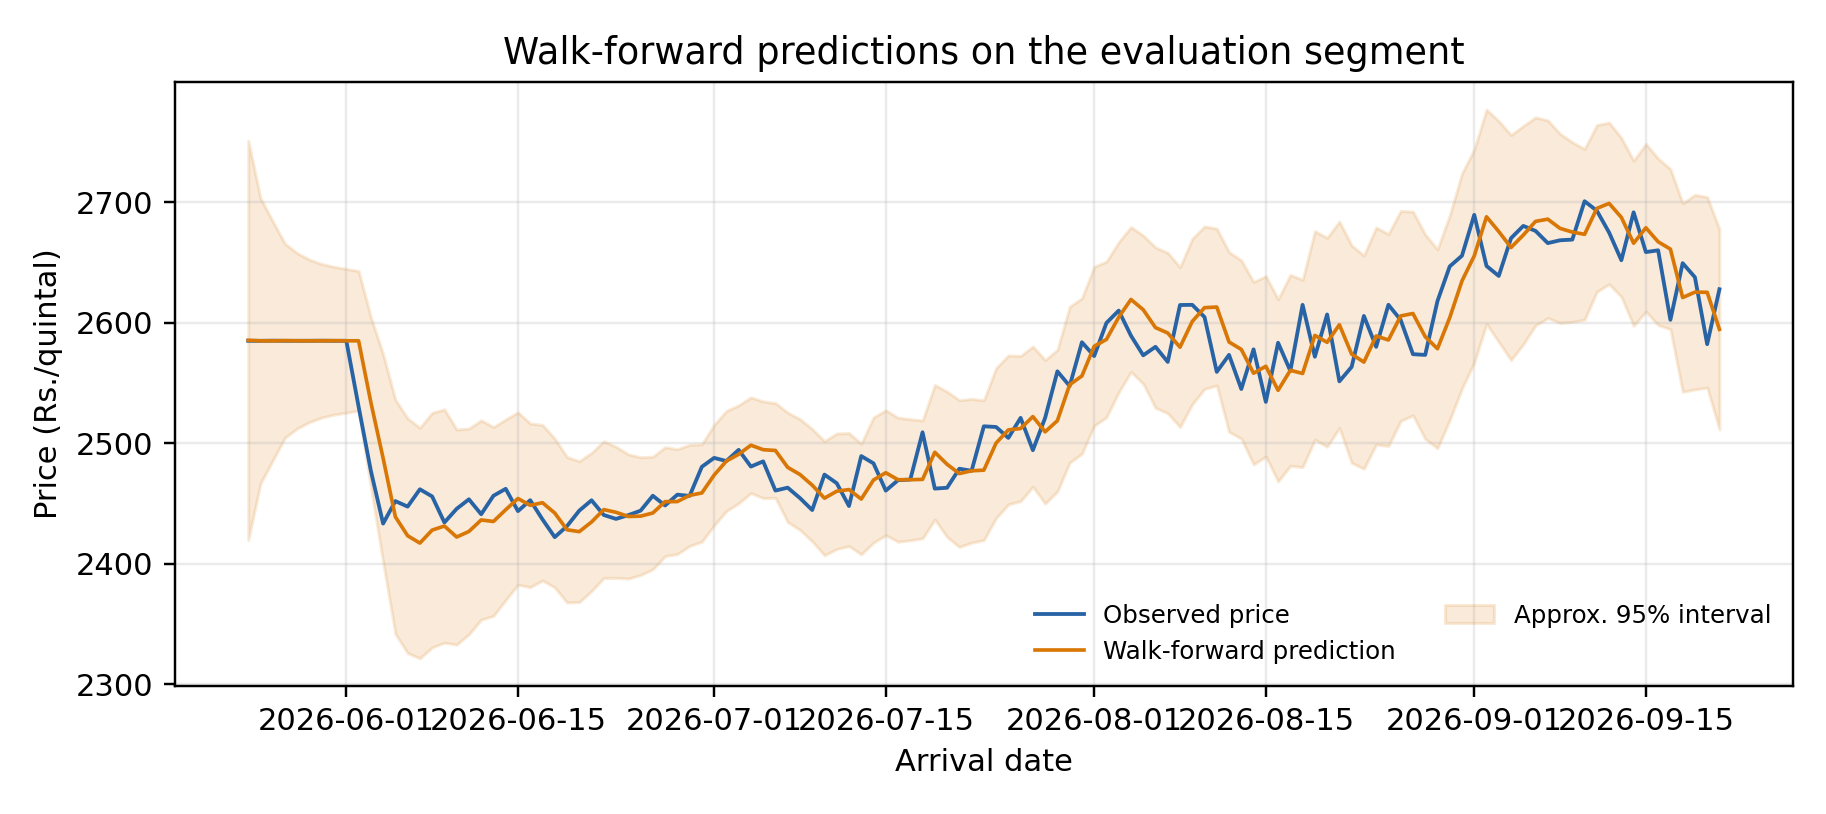
\includegraphics[width=0.98\textwidth]{02_walk_forward_test.png}
\caption{Observed prices, gap-aware walk-forward forecasts, and approximate 95\% predictive intervals on the evaluation segment.}
\label{fig:testfit}
\end{figure}

\section{Innovation diagnostics}
Figure~\ref{fig:innovation} plots the signed innovations during the evaluation segment. If the model were well calibrated, errors would ideally be centred around zero and would not display long systematic runs of one sign. Strong serial structure in the innovations would suggest that the state dynamics omit useful information. Large isolated innovations can indicate unexpected market shocks, changes in the mix of varieties, recording issues, or model misspecification; the time series alone does not identify the cause.

\begin{figure}[H]
\centering
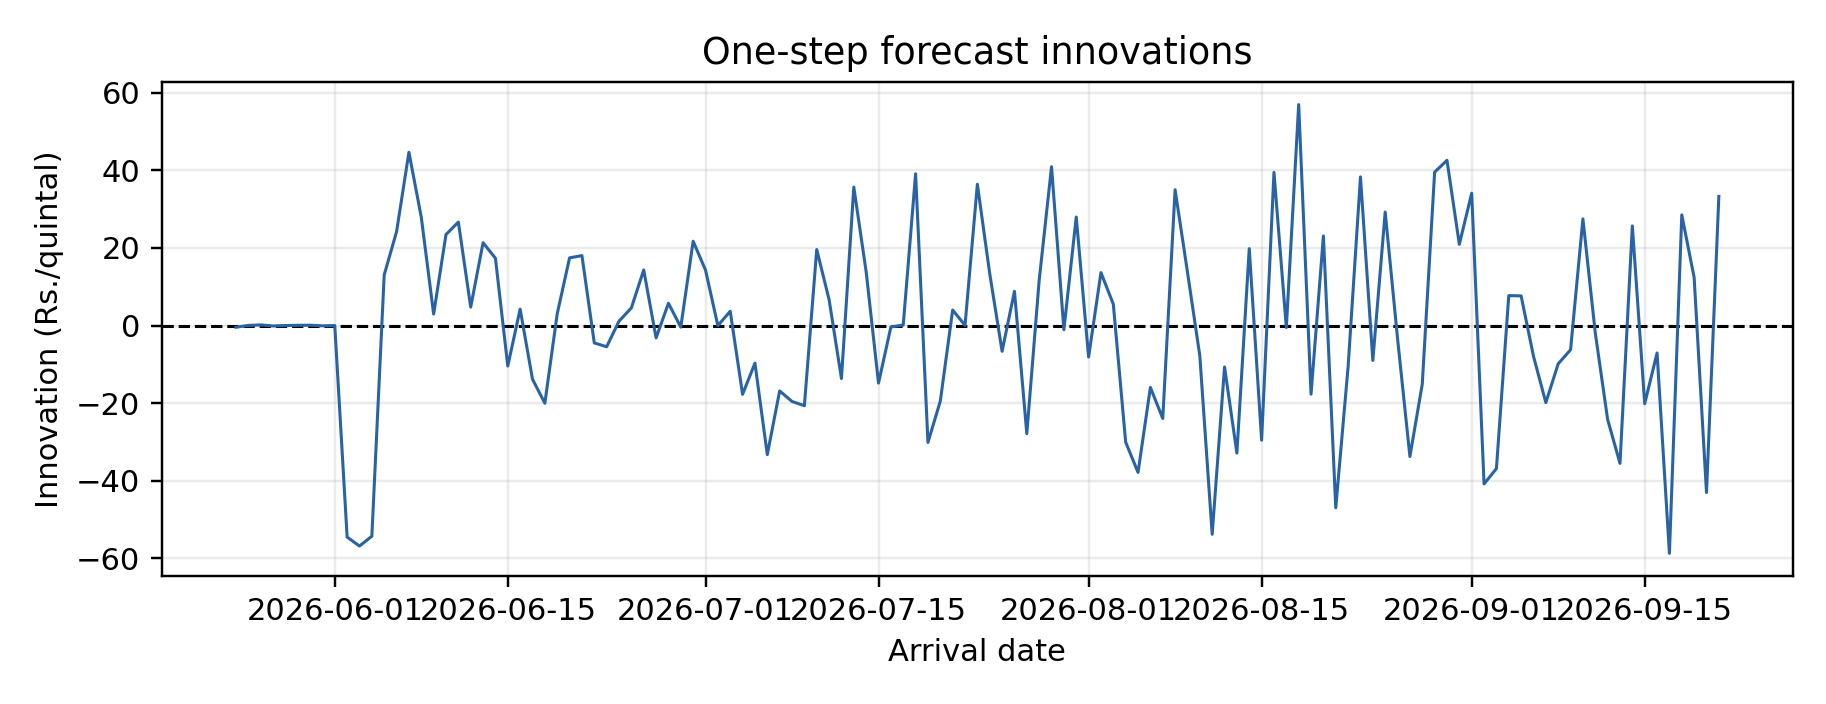
\includegraphics[width=0.98\textwidth]{03_innovations.png}
\caption{Signed innovations, defined as actual price minus its prior forecast.}
\label{fig:innovation}
\end{figure}

\section{Kalman gain diagnostics}
Figure~\ref{fig:gain} displays the level component of the gain. This number describes how strongly the observed price corrects the predicted level on a given step. It should not be interpreted as a probability. A gain close to one means that, in the scalar-level intuition, much of the innovation is incorporated; a smaller gain means that the correction is more conservative. The actual two-state gain is a vector, so the trend component also matters for the full state update.

\begin{figure}[H]
\centering
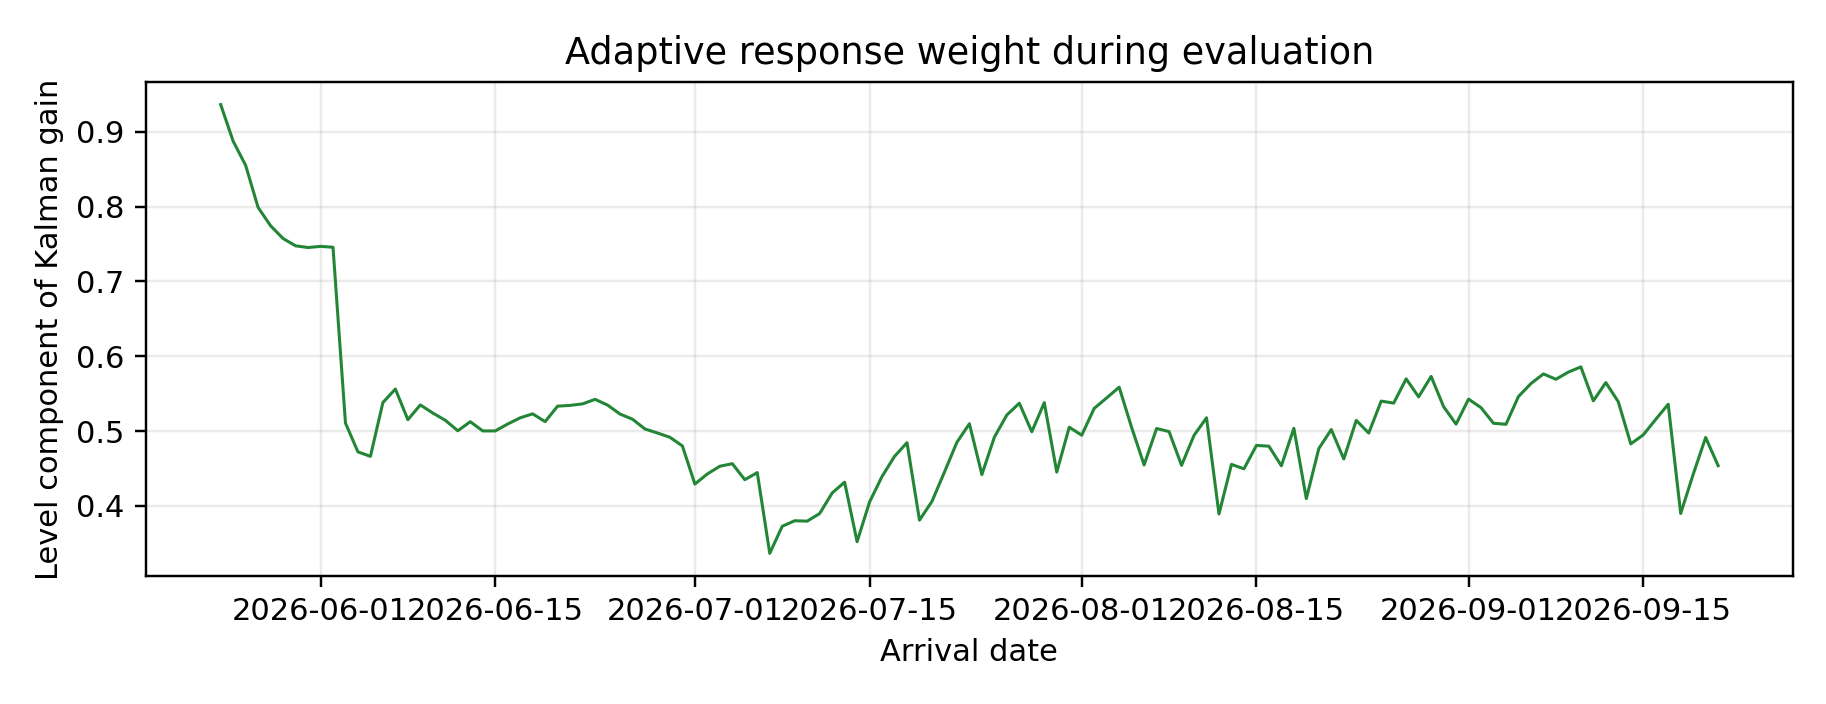
\includegraphics[width=0.98\textwidth]{04_kalman_gain.png}
\caption{Level component of the Kalman gain through the evaluation period.}
\label{fig:gain}
\end{figure}

\section{One forecast at the dataset cutoff}
For illustration, running the online state update through all 221 observations and then propagating the filtered state by one calendar day gives a next-day point forecast of approximately Rs.\ 2,602.81 per quintal. Using the model's Gaussian-style predictive standard deviation gives an approximate interval from Rs.\ 2,517.77 to Rs.\ 2,687.86 per quintal. This is an offline calculation based on a dataset whose last observation is 21 September 2026; it is not presented as a current price or a forecast for today's market. It simply illustrates how the equations produce a point estimate and an uncertainty range at the end of the file.

% ============================== CHAPTER 7 ==============================
\chapter{Implementation, Assumptions, and Limitations}

\section{Basic website architecture}
The website is a presentation layer for exploring the selected historical price series and viewing its forecast. Its current prototype is a small client-server application: the browser presents the controls and plots, while a Python backend filters the CSV data, constructs the target series, runs the forecasting algorithm, and returns structured results. The website does not change the underlying mathematics; it provides a convenient way to choose inputs and display the result.

\begin{figure}[H]
\centering
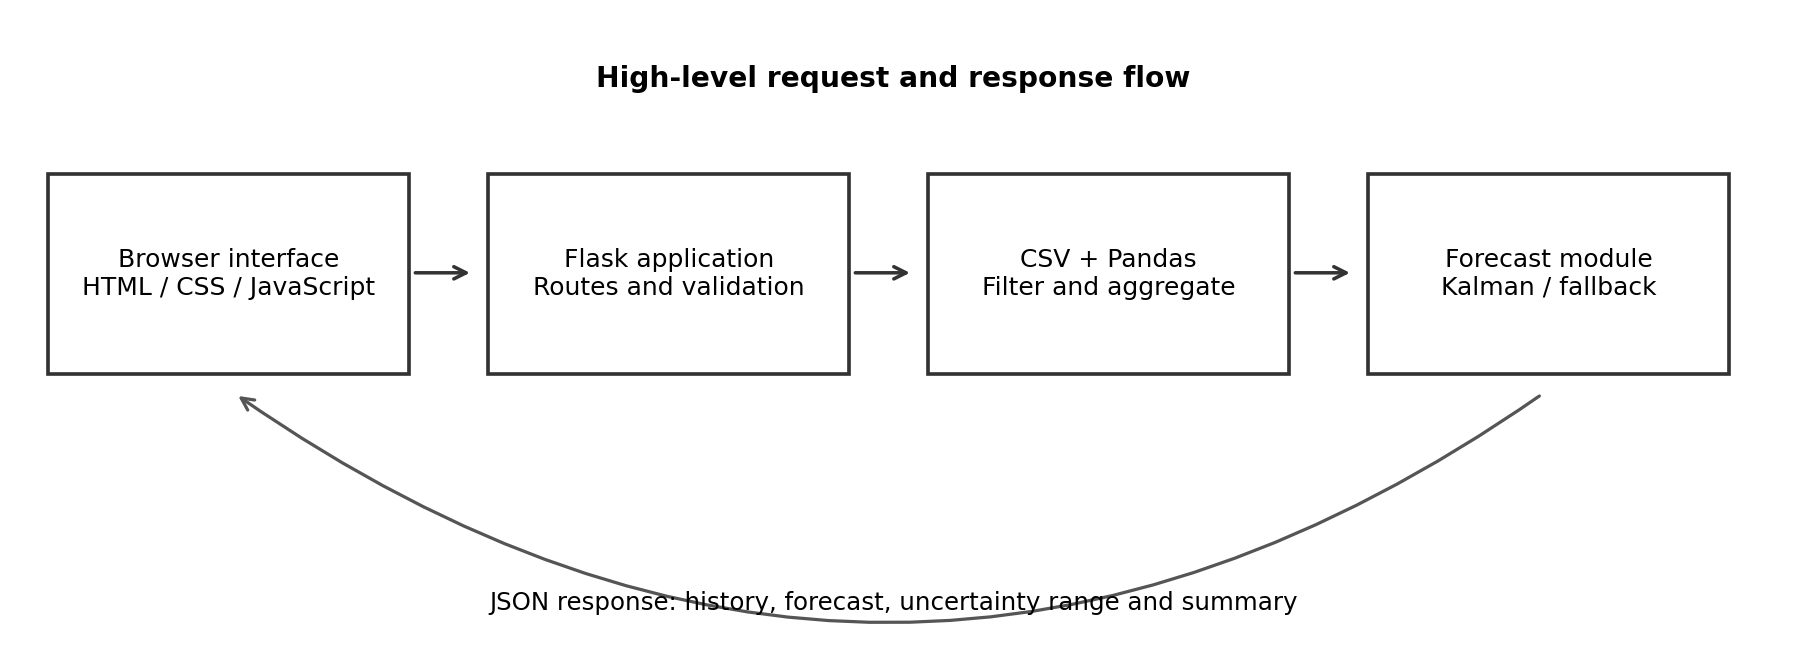
\includegraphics[width=0.98\textwidth]{06_website_architecture.png}
\caption{High-level architecture of the CSV-backed forecasting website. Requests move from the browser to the Flask backend; the backend filters the local data, runs the selected-series forecast, and returns a JSON response for display.}
\label{fig:websitearchitecture}
\end{figure}

\subsection{Presentation layer: the user's browser}
The browser loads the HTML page from \path{templates/index.html}, while \path{static/style.css} controls layout, typography, responsive behaviour, and colours. The JavaScript file \path{static/app.js} handles filter changes, sends requests to the backend, and draws the historical and forecast chart using Chart.js. The interface includes filters for state, district, market, commodity, variety, and grade, along with a forecast horizon. Only options found in the currently loaded dataset can appear in these controls. In the present CSV snapshot, the commodity available is wheat and the variety dimension contains multiple wheat varieties.

\subsection{Application layer: Flask routes}
The Python application in \path{app.py} uses Flask to serve the page and expose small JSON endpoints. The route \texttt{/} returns the interface. The route \texttt{/api/options} supplies the available filter options, \texttt{/api/summary} returns basic counts and the latest date in the loaded file, and \texttt{/api/forecast} accepts the current filters and the requested forecast horizon and returns the results. If the selected filters do not match any valid records, the backend returns an error message so the user can choose a broader selection.

\subsection{Data and forecasting layer}
At application startup, the CSV is read into a Pandas DataFrame held in memory. Numeric price and arrival columns are parsed, dates are interpreted, and filter fields are cleaned. For a request, the backend applies the selected filters and groups the matching records by arrival date. Modal prices are combined using the arrival-weighted mean when positive arrival weights are available; if the weights sum to zero, the implementation uses the unweighted mean of valid quotations. The current CSV contains only Wheat, so date grouping cannot mix different crop names in this experiment. If additional commodities are added, the backend should require an explicit commodity selection or generate one independent series per commodity; it must not average unrelated commodities into a single target. Thus, the report distinguishes the reusable design from empirically verified performance on the present wheat case study.

The resulting date-ordered series is passed to the adaptive, gap-aware Kalman forecasting routine. When sufficient history is available, the routine estimates the local price level and trend and generates future values and approximate uncertainty bounds. For selections with fewer than 20 observed dates, the current prototype uses a simple previous-price fallback and displays a notice that the history is limited. The backend returns the historical observations, predictions, relevant summary values, model name, and evaluation metrics (when enough data are available) in JSON format.

\subsection{Request-response flow}
The interaction can be summarized as follows:
\begin{enumerate}
  \item The user chooses a market, commodity, variety, grade, and forecast horizon in the browser.
  \item The browser requests available filter options or a forecast from a Flask endpoint.
  \item The backend applies the filters to the in-memory CSV data and builds a separate daily series for that selection.
  \item The forecasting routine returns future estimates and uncertainty ranges, or a previous-price fallback for a very short series.
  \item The backend sends a JSON response and the browser refreshes the chart, forecast table, and plain-language summary.
\end{enumerate}

\subsection{Current scope and future integration}
The current version uses a local CSV snapshot loaded when the Python process starts. It is not yet connected to a live market-data API, web scraper, persistent database, login system, or scheduled update service. Adding these capabilities would require a separate ingestion and validation layer, secure configuration for credentials, storage of verified observations, and monitoring of data freshness and failed updates. These are future engineering tasks; the results in Chapter~6 come from the offline data snapshot and do not rely on live updates.

\section{Computational implementation}
The data pipeline is implemented using Python. Pandas parses the CSV, converts relevant columns to numeric and datetime types, handles invalid rows, groups observations by date, and sorts the series. NumPy performs the weighted aggregation and matrix calculations. Matplotlib generates the diagnostic plots. The core numerical algorithm requires only two state coordinates and small matrices, so each filtering step is computationally inexpensive.

The algorithm stores the state estimate $\hatt{x}_{t|t}$, the covariance $P_{t|t}$, the current process-noise covariance $Q_t$, and observation-noise variance $R_t$. At each subsequent observation it performs one prediction and one correction. For a two-dimensional state, the matrix operations are constant-sized; the overall time cost grows linearly in the number of observations, $O(n)$, and memory use for online operation can be constant apart from optional stored predictions and plotting arrays.

\section{Model assumptions}
The main assumptions can be summarized as follows:
\begin{enumerate}
  \item The current target price is an observation of a latent price level plus observation noise.
  \item The latent level evolves locally according to the previous level and trend.
  \item The trend is locally persistent but may change through process noise.
  \item Process and observation noises are zero-mean and treated as mutually uncorrelated in the Kalman derivation.
  \item A linear-Gaussian approximation is adequate for constructing the recursive estimates, although market shocks need not be Gaussian in reality.
  \item The parameters chosen for initialization and noise adaptation are reasonable numerical heuristics for the available sample.
\end{enumerate}

\section{Limitations}
\subsection{Single market and short history}
The numerical case study represents one market in one district and one commodity (wheat) for a period of less than a year. The 221 observations are not enough to establish that the same dynamics hold across other commodities, varieties, Indian mandis, or seasons. Generalization requires records from additional commodities and markets and a longer history. Although the website filter design is reusable, a selection can only be forecast when the underlying dataset contains sufficient valid observations for it.

\subsection{Mixed-variety target}
The target is constructed from the records matching the selected commodity and market filters. When all varieties of one commodity are selected, the date-level target is an arrival-weighted mean across those varieties. Its value changes not only when each variety's price changes, but also when the arrival mix changes. A fixed-variety forecast such as Dara has a different interpretation and empirical distribution from an all-variety indicator. The model must be run separately for each selected commodity or variety; prices from distinct commodities should never be aggregated into a single target. Evaluation should state the exact selection used.

\subsection{No explicit seasonal or exogenous component}
The model includes a local level and trend but no weekly, harvest, festival, or annual seasonal state. It also does not include explanatory predictors such as arrivals, weather, minimum support price, fuel cost, or neighbouring-market prices. If such factors influence prices, their effects may appear as unexplained innovations.

\subsection{Heuristic noise adaptation}
The values 0.20, 0.02, 0.15, 0.85, and the variance floors are design choices. They are not estimated by maximizing a likelihood or minimizing an objective over rolling validation windows. The adaptive $R_t$ uses squared forecast innovations, which combine measurement noise and process-model errors. The adaptive $Q_t$ uses recent differences but does not normalize them by elapsed calendar time. These details are important if the method is refined.

\subsection{Uncertainty intervals are approximate}
The interval in Equation~\eqref{eq:interval} assumes a well-calibrated predictive variance and approximately Gaussian error. The project does not claim to have established 95\% empirical coverage. Future evaluations should report the fraction of held-out observations falling within the predicted interval, average interval width, and an interval scoring rule.

\subsection{Small margin over persistence}
The previous-price baseline already performs well because many prices change gradually. The gap-aware Kalman filter slightly improves the summary metrics on this sample. To verify that this improvement is robust, it should be repeated across multiple chronological origins, with sensitivity analysis for training-window length and model noise settings.

\section{Future directions}
Several extensions are mathematically natural.
\begin{itemize}
  \item \textbf{Systematic parameter calibration:} select noise scales using a validation window or maximize the likelihood of the one-step innovations. Any tuning must preserve the chronological train-validation-test separation.
  \item \textbf{Gap-consistent process noise:} derive $Q(\Delta_t)$ from an explicit continuous-time local-trend process or normalize price differences by elapsed time before estimating recent volatility.
  \item \textbf{Seasonal state-space components:} include weekly patterns or longer seasonal dynamics if longer historical records provide evidence for them.
  \item \textbf{Exogenous variables:} add market arrivals, neighbouring-market prices, weather summaries, or policy variables when reliable data and a defensible causal/predictive design are available.
  \item \textbf{Broader evaluation:} use rolling-origin evaluation and compare with persistence, moving averages, exponential smoothing, and appropriately specified ARIMA models.
  \item \textbf{Interval calibration:} evaluate coverage and width of predictive intervals rather than relying only on point-error metrics.
  \item \textbf{Multi-commodity validation:} include sufficiently long histories for additional crops and markets, run a separate series and evaluation for each selected item, and report results by commodity rather than pooling unrelated prices.
  \item \textbf{Operational data pipeline:} connect the interface to a verified data source, record data freshness and ingestion errors, and monitor the model on newly observed prices. This is future deployment work, not part of the offline metrics presented here.
\end{itemize}

% ============================== CHAPTER 8 ==============================
\chapter{Conclusion}
This project develops a reusable framework for constructing a chronological price series for a selected agricultural commodity or variety and applying an adaptive, gap-aware Kalman filter to estimate its hidden price level and local trend. The supplied dataset supports a wheat case study at Kanpur (Grain) APMC; therefore, the quantitative results reported here should be read as a demonstration on that dataset, rather than as evidence of accuracy across all crops. The report begins with the definitions needed to understand the task: time index, lag, first difference, mean, median, sample variance, random variables, covariance matrices, and state-space representation. It then derives the prediction and correction steps of the Kalman filter, explains how the Kalman gain combines a prior estimate with new evidence, and describes how the implementation updates its process and observation noise scales.

The main target contains 221 observed date-level prices built from 870 valid source rows. The model is initialized from 100 observations and evaluated on the next 121 observations in chronological walk-forward order. The adaptive gap-aware filter achieves MAE of Rs.\ 18.871 per quintal, RMSE of Rs.\ 24.337 per quintal, and MAPE of 0.7404\%, compared with 0.7456\% MAPE for a previous-price baseline. This is a modest improvement on the given data and should be interpreted as evidence about this experiment rather than a universal guarantee.

The central lesson is that a forecasting result depends on more than its final error metric. The definition of the target, date gaps, ordering of prediction and update, assumptions about uncertainty, baseline choice, and evaluation protocol all affect whether a result is meaningful. The current model is lightweight and mathematically interpretable, but it omits explicit seasonality and external predictors and uses heuristic noise adaptation. Longer data histories, rigorous calibration, rolling-origin validation, and empirical interval checks are the main next steps toward a more reliable forecasting system.

% ============================== APPENDIX ===============================
\appendix
\chapter{Notation and Equation Summary}
\begin{longtable}{@{}p{0.22\textwidth}p{0.72\textwidth}@{}}
\toprule
Symbol & Meaning \\
\midrule
\endfirsthead
\toprule
Symbol & Meaning \\
\midrule
\endhead
$y_t$ & Observed arrival-weighted modal price on observed date $d_t$. \\
$d_t$ & Calendar date associated with observation index $t$. \\
$\Delta_t$ & Number of elapsed calendar days between $d_{t-1}$ and $d_t$, with a minimum value of 1. \\
$x_t=[\ell_t,b_t]\trans$ & Hidden state containing price level and local trend. \\
$F_t$ & State-transition matrix $\begin{bmatrix}1&\Delta_t\\0&1\end{bmatrix}$. \\
$H$ & Observation matrix $[1\;0]$, selecting the level. \\
$w_t,Q_t$ & Process disturbance and its covariance matrix. \\
$v_t,R_t$ & Observation disturbance and its variance. \\
$\hatt{x}_{t|t-1}$ & Prior state estimate before using the current observation. \\
$P_{t|t-1}$ & Prior covariance of the state estimation error. \\
$e_t$ & Innovation, equal to $y_t-\hatt{y}_{t|t-1}$. \\
$S_t$ & Innovation variance, $HP_{t|t-1}H\trans+R_t$. \\
$K_t$ & Kalman gain vector. \\
$\hatt{x}_{t|t},P_{t|t}$ & Updated state estimate and posterior error covariance. \\
$\operatorname{MAE}$ & Mean absolute error. \\
$\operatorname{RMSE}$ & Root mean squared error. \\
$\operatorname{MAPE}$ & Mean absolute percentage error. \\
\bottomrule
\end{longtable}

\chapter{A Worked One-Step Kalman Update}
This appendix evaluates the filter's first test step using the numerical values obtained from the supplied dataset. It is included to connect the matrix equations to actual calculations. The last training observation is dated 23 May 2026, the first evaluation observation is dated 24 May 2026, and hence $\Delta_t=1$ for this example.

The initial variance scale is $s_0^2=3043.7157$. The initialized state and matrices are
\[
\hatt{x}_{t-1|t-1}=\begin{bmatrix}2585.3152\\0.1360\end{bmatrix},\quad
P_{t-1|t-1}=\begin{bmatrix}3043.7157&0\\0&3043.7157\end{bmatrix},
\]
\[
Q_0=\begin{bmatrix}608.7431&0\\0&60.8743\end{bmatrix},\qquad R_0=456.5574,
\]
where price is measured in Rs. per quintal and the trend is represented numerically as a daily change. Since the date gap is one day,
\[
F_t=\begin{bmatrix}1&1\\0&1\end{bmatrix}.
\]
The prior state follows from matrix multiplication:
\[
\hatt{x}_{t|t-1}=F_t\hatt{x}_{t-1|t-1}
=\begin{bmatrix}2585.4512\\0.1360\end{bmatrix}.
\]
The prior covariance and innovation variance are
\[
P_{t|t-1}=F_tP_{t-1|t-1}F_t\trans+Q_0
=\begin{bmatrix}6696.1745&3043.7157\\3043.7157&3104.5900\end{bmatrix},
\]
\[
S_t=(P_{t|t-1})_{11}+R_0=6696.1745+456.5574=7152.7319.
\]
The Kalman gain is therefore
\[
K_t=\frac{1}{7152.7319}\begin{bmatrix}6696.1745\\3043.7157\end{bmatrix}
=\begin{bmatrix}0.93617\\0.42553\end{bmatrix}.
\]
The actual observed price on 24 May 2026 is $y_t=2585.0000$, so the innovation is
\[
e_t=2585.0000-2585.4512=-0.4512.
\]
The corrected state is
\[
\hatt{x}_{t|t}=\hatt{x}_{t|t-1}+K_te_t
\approx\begin{bmatrix}2585.0288\\-0.0560\end{bmatrix}.
\]
In this step, the observation is only slightly below the prior forecast, so the estimated level decreases by about Rs.\ 0.4224 per quintal. The negative innovation also lowers the trend estimate. The posterior covariance obtained from the implemented simplified update is approximately
\[
P_{t|t}\approx\begin{bmatrix}427.4154&194.2797\\194.2797&1809.3918\end{bmatrix}.
\]
Finally, the observation-noise adaptation uses the squared innovation but enforces a floor of $0.05s_0^2$. Since $0.05s_0^2\approx152.1858$ is larger than $e_t^2$, the next observation-noise variance is
\[
R_{t+1}=0.85(456.5574)+0.15(152.1858)\approx410.9016.
\]
This example illustrates the entire sequence: transition, uncertainty propagation, innovation calculation, gain calculation, state correction, covariance correction, and noise adaptation. The forecast of Rs.\ 2,585.4512 is recorded before the actual Rs.\ 2,585.0000 observation is used.

\chapter{Pseudocode for the Main Filter}
The following pseudocode emphasizes the order of operations. The forecast must be saved before the current observation is incorporated.
\begin{lstlisting}[language=Python,caption={High-level adaptive gap-aware Kalman recursion}]
Initialize level x[0], trend x[1], covariance P
Initialize process covariance Q and observation variance R

for each observed date t after the first 100 observations:
    dt = max(calendar_days(date[t] - date[t-1]), 1)
    F = [[1, dt], [0, 1]]

    x_pred = F @ x
    P_pred = F @ P @ transpose(F) + Q * dt
    y_pred = x_pred[0]
    S = P_pred[0,0] + R
    K = P_pred[:,0] / S

    save y_pred before reading this date's value into the filter
    innovation = y[t] - y_pred
    x = x_pred + K * innovation
    P = P_pred - outer(K, P_pred[0,:])
    P = (P + transpose(P)) / 2

    R = 0.85 * R + 0.15 * max(innovation**2, 0.05 * initial_var)
    if enough recent observations exist:
        recent_var = sample_variance(recent first differences)
        Q[0,0] = 0.20 * recent_var
        Q[1,1] = 0.02 * recent_var
\end{lstlisting}

\chapter{Reproducibility Notes}
The numerical values reported in Chapter~6 are based on the supplied wheat case-study file and the following modelling choices: (i) the selected wheat variety records are combined into an arrival-weighted date-level modal price; (ii) the observations are sorted in ascending date order; (iii) the first 100 observations initialize the filter; (iv) the following 121 observations are evaluated sequentially; (v) the gap-aware transition and $\Delta_tQ_t$ covariance scaling are used; (vi) adaptive noise updates are applied after each observed test price; and (vii) the naive benchmark uses the preceding observed price.

For reproducibility, the implementation should retain the original CSV alongside the source code, record any changes to date parsing or aggregation, and recompute all metrics whenever the data or filter constants change. The dataset ends on 21 September 2026, so all values in this report are tied to that historical snapshot.

% ============================= BIBLIOGRAPHY ============================
\begin{thebibliography}{9}
\addcontentsline{toc}{chapter}{Bibliography}

\bibitem{kalman1960}
R. E. Kalman,
\emph{A New Approach to Linear Filtering and Prediction Problems},
Journal of Basic Engineering, vol. 82, no. 1, pp. 35--45, 1960.
\url{https://doi.org/10.1115/1.3662552}.

\bibitem{welch2006}
G. Welch and G. Bishop,
\emph{An Introduction to the Kalman Filter},
Technical Report TR 95-041, Department of Computer Science, University of North Carolina at Chapel Hill, revised 2006.
\url{https://www.cs.unc.edu/~welch/media/pdf/kalman_intro.pdf}.

\bibitem{durbin2012}
J. Durbin and S. J. Koopman,
\emph{Time Series Analysis by State Space Methods}, 2nd ed.,
Oxford University Press, 2012.
\url{https://doi.org/10.1093/acprof:oso/9780199641178.001.0001}.

\bibitem{hyndman2021}
R. J. Hyndman and G. Athanasopoulos,
\emph{Forecasting: Principles and Practice}, 3rd ed., OTexts, 2021.
\url{https://otexts.com/fpp3/}.

\bibitem{hamilton1994}
J. D. Hamilton,
\emph{Time Series Analysis}, Princeton University Press, 1994.

\bibitem{projectdata}
Project dataset,
\emph{Daily Price Arrival Report: 07-11-2025 to 21-09-2026 for Uttar Pradesh},
CSV file supplied for this project. The actual first valid observed date in the cleaned rows is 11 November 2025.

\end{thebibliography}

\end{document}
